\subsection{Lecture de tension des modules}
	\paragraph*{}
	La majorité de l'information sur la batterie provient de la tension des modules, c'est pourquoi cette mesure doit être très précise et robuste sur toute la plage d'utilisation des modules. Le circuit doit consommer un minimum de courant, être robuste, modulable et précis. Le circuit doit aussi faciliter la vérification technique.
	
	\subsubsection*{Solution commerciale}
	\paragraph*{}
	Il existe sur le marché plusieurs circuits qui s'occupent de lire la tension des modules et de communiquer l'information à un microcontrôleur. Les fonctionnalités et le nombre de modules supportés varient d'un vendeur à l'autre. Les points communs sont : 

	\begin{multicols}{2}
		\begin{itemize}
			\item[$\bullet$] Le circuit peut être alimenté par les modules;
			\item[$\bullet$] Consommation de courant de quelque mA lorsque le circuit prend les mesures et quelques $\mu$A lorsqu'il est en veille;
			\item[$\bullet$] Solution compacte;
			\item[$\bullet$] Lecture précise;
			\item[$\bullet$] Les modules doivent être branchés dans l'ordre;
			\item[$\bullet$] Économique;
			\item[$\bullet$] Fonctionnement bien documenté.
		\end{itemize}
	\end{multicols}

	\paragraph*{}
	Cette solution est réalisable et demande surtout de bien lire et comprendre la documentation. Le LTC6804 de Linear Technology a été retenu pour son nombre de modules maximum, son prix et sa simplicité d'implémentation. Cette solution répond à la majorité des spécifications, mais elle n'apporte cependant rien de nouveau au système actuellement utilisé et elle ne facilite pas la vérification technique. 
	

	
	\subsubsection*{Isolation des lectures}
	\paragraph*{}
	La vérification technique sera beaucoup plus facile si les différentes lectures de tensions sont isolées. Ce point est décrit dans la section Manipulations et vérifications techniques. 
	
	\paragraph*{}
	L'isolation amène plusieurs avantages :
	
	\begin{itemize}
		\item[$\bullet$] Les modules n'ont plus besoin d'être branchés en ordre, ce qui élimine le risque d'erreur humaine;
		\item[$\bullet$] Il est possible de débrancher une seule cellule pour venir ensuite la remplacer par une alimentation variable;
		\item[$\bullet$] Le filage dans la batterie peut être mieux organisé et optimisé.
	\end{itemize}

	\paragraph*{}
	Cette solution comporte cependant plusieurs désavantages :
	
	\begin{itemize}
		\item[$\bullet$] Consomme plus de courant (quelque mA par module lors des lectures);
		\item[$\bullet$] Demande plus de composantes;
		\item[$\bullet$] Plus difficile à implémenter;
		\item[$\bullet$] Plus dispendieux.
	\end{itemize}
	
	\paragraph*{}
	Ces différents désavantages ne sont pas majeurs dans le contexte d'Éclipse, la consommation de courant reste insignifiante comparée à ce que le moteur et le reste des circuits consomment. Le nombre de composants peut être limité en utilisant la bonne topologie et le prix de la carte peut être plus élevé tant qu'il respecte le budget. 
	
	\subsubsection*{Circuit analogique}
	\paragraph*{}
	Une solution relativement simple et qui ne comporte pas beaucoup de composantes est montrée à la figure \ref{fig:HCNR201}. Ce circuit très compact et simple n'est pas assez précis puisque le gain entre les deux photodiodes varie de 5\% pour le HCNR201. Cette erreur ne répond pas aux spécifications de +/- 10mV qui représente une erreur de $\pm 0.238 \%$ ($\pm 10mV / 4.2V \cdot 100 \%$).  
	
	\begin{figure}[H]
		\centering
		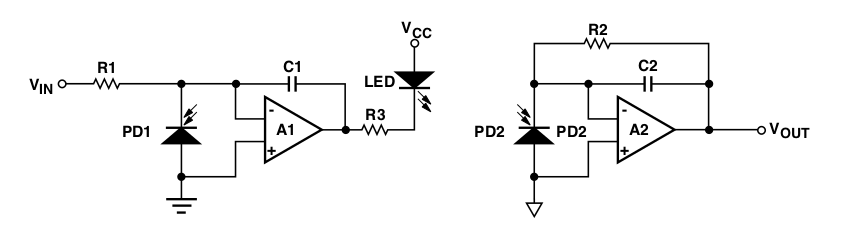
\includegraphics[scale = 0.5]{Images/Analogique.png}
		\caption{Circuit de lecture de tension isolée analogique \cite{HCNR201}}
		\label{fig:HCNR201}
	\end{figure}

	\subsubsection*{Lecture d'un voltage de référence avec un ADC}
	\paragraph*{}	
	Pour éliminer l'erreur causée par l'amplificateur et l'isolateur tout en réduisant au maximum le nombre de composants, l'ADC mesurerait un voltage de référence alors qu'il serait alimenté par le module comme présenté à la figure \ref{fig:adc_vref}. Puisque le voltage à l'entrée est connu, la tension du module est donnée par l'équation \ref{eq:vref}.
	
	\begin{align}
		V_{Module} = \dfrac{V_{REF}}{Valeur~ADC} \cdot 2^{~nb~Bits~adc}
		\label{eq:vref}
	\end{align}
	
	\begin{figure}[H]
		\centering
		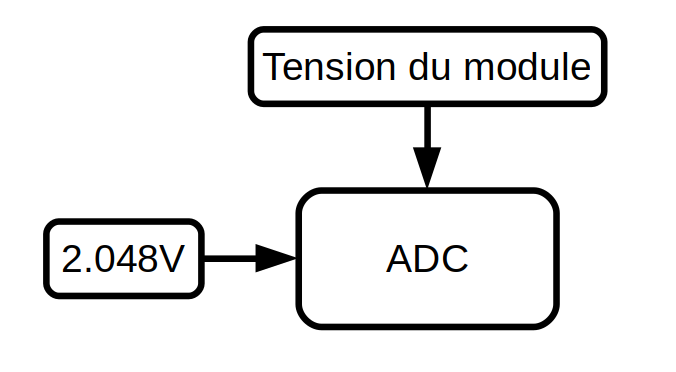
\includegraphics[scale=0.3]{Images/Voltage_reference.png}
		\caption{Lecture d'un voltage de référence avec un ADC}
		\label{fig:adc_vref}
	\end{figure}
	
	\paragraph*{}
	Le circuit mesure le LSB qui est donné par $V_{Module} / 2^{~nb~Bits~adc}$ pour  trouver la tension du module. Bien que cette technique fonctionne, les courbes de la tension du module et de la résolution ne sont pas linéaires par rapport au résultat du ADC. La valeur du voltage de référence à un impacte sur la courbe de la résolution. Plus il est bas, moins la courbe est linéaire et la résolution est moins bonne. Les figures \ref{fig:vmodule_vref} et \ref{fig:res_vref} montrent les performances idéales du circuit à la figure \ref{fig:adc_vref} avec une référence de 2.048V et une plage de 2V à 4.2V pour la tension du module.
	
	\begin{figure}[H]
		\begin{minipage}{0.45\textwidth}
			\centering
			\fbox{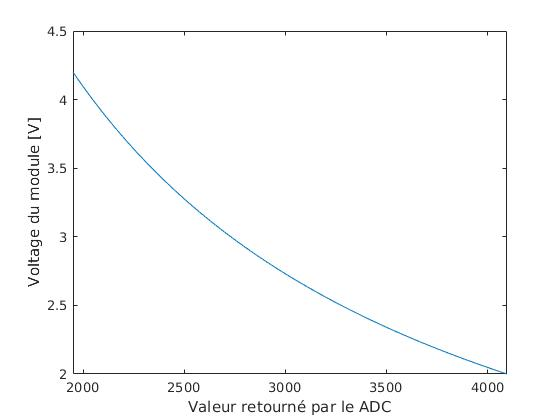
\includegraphics[scale=0.4]{Images/Vmodule_REF_2V.jpg}}
			\caption{Tension du module en fonction des valeurs du ADC}
			\label{fig:vmodule_vref}
		\end{minipage}
		\hfill
		\begin{minipage}{0.45\textwidth}
			\centering
			\fbox{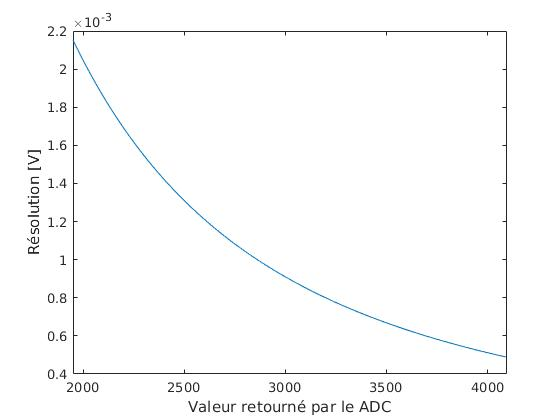
\includegraphics[scale=0.4]{Images/RES_REF_2V.jpg}}
			\caption{Résolution en fonction des valeurs du ADC}
			\label{fig:res_vref}
		\end{minipage}	
	\end{figure}	
	
	\paragraph*{}
	L'écart maximal entre 2 bits est de 2.15 mA. Avec un ADC performant qui a une erreur de $\pm 1$ LSB, la lecture de tension à une erreur maximale de $\pm $ 2.15 mA lorsque le module est à 4.2V. Cette méthode correspond à la spécification qui demande d'être à $\pm $ 10 mA. L'ADC consomme et la tension de référence consomme très peu de courant, ils nécessitent très peu de composants externes et ils sont abordables. Afin d'avoir une très bonne précision, il est nécessaire de faire une calibration puisque la tolérance de la référence ($\pm$ 0.5 \%) est plus grande que celle de la spécification ($\pm 0.238 \%$). Il existe des références avec des tolérances plus petites que $\pm 0.238 \%$ mais elles sont beaucoup trop dispendieuses pour le projet puisqu'il faut en avoir une pour chaque module.    
	
	\paragraph*{}
	L'isolation de la mesure se fait au niveau de la communication puisqu'il n'y a aucune erreur causée par l'isolateur de cette façon, contrairement à l'optocoupleur de la solution analogique. L'alimentation de l'isolateur et du ADC doit dépasser la plage de lecture du module qui est de 2V à 4.5V.
	
	\paragraph*{}
	Cette solution est viable, elle respecte les spécifications et elle ne demande pas beaucoup de composantes. Le choix des ADC et des isolateurs numériques avec une alimentation qui va de moins de 2V à plus de 5V est toutefois très restreint. Les prix de l'isolateur et de l'ADC sont donc élevés et il est plus difficile de trouver un remplacement dans le cas ou un composant n'est plus disponible.   
	
	\subsubsection*{Configuration classique d'un ADC}
	\paragraph*{}
	Pour utiliser l'ADC avec une configuration classique où l'entrée mesure le voltage du module, un convertisseur de puissance est nécessaire pour maintenir une tension fixe qui est plus élevée que celle du module. Plusieurs composants externes sont nécessaires, mais les coûts sont absorbés par le prix moins élevé de l'ADC et de l'isolateur. Cette topologie permet d'avoir une résolution qui est fixe sur toute la plage des mesures, un contrôle sur le LSB avec l'alimentation de l'ADC et un meilleur choix d'ADC. Le ADC est alimenté par un régulateur linéaire pour avoir un minimum de bruit alors que l'isolateur est alimenté par le convertisseur à commutation. L'isolateur qui commute rapidement ne vient donc pas perturber l'alimentation de l'ADC. Puisque l'alimentation de l'ADC  est utilisée comme référence, il est important de faire une calibration pour avoir un LSB qui est très précis afin d'avoir une mesure qui respecte les spécifications. Avec la référence calibrée à 4.5V et un ADC qui à une erreur de $\pm$ 1 LSB, la précision de la mesure est de $\pm 1.1$ mV sur toute la plage. La tension du module est donnée par l'équation \ref{eq:Vmodule}.
	
	\begin{align}
		V_{Module} = \dfrac{V_{Ref}}{2^{~nb~Bits~adc}} \cdot \text{Valeur ADC}
		\label{eq:Vmodule}
	\end{align}
	
	\begin{figure}[H]
		\centering
		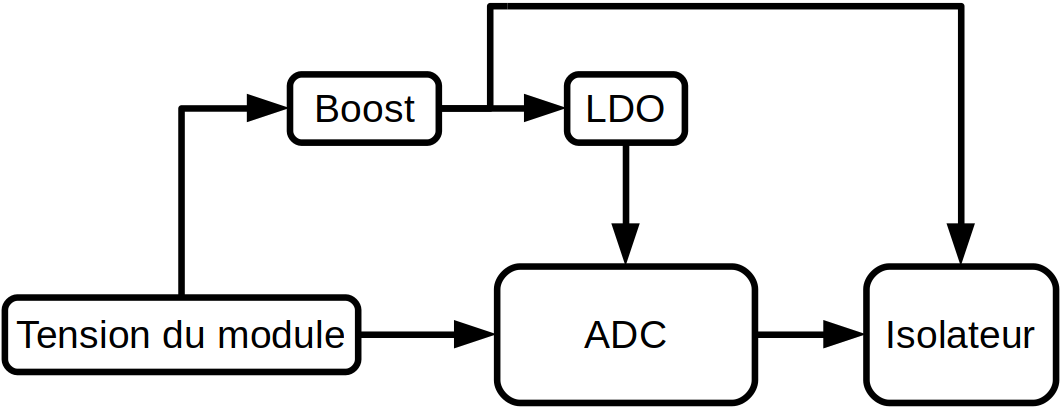
\includegraphics[scale=0.3]{Images/Tension_module.png}
		\caption{Lecture de la tension du module}
		\label{fig:adc_vmod}
	\end{figure}	

	\paragraph*{}
	Le nombre de composants rend cette solution plus dure à implémenter en raison de l'espace restreint que les modules esclaves peuvent prendre dans la batterie. Les composants devront être choisis en fonction de leurs performances et leur format. Cette topologie offre de bonnes performances et elle n'est pas plus dispendieuse que la solution précédente. 
	
	\subsubsection*{Choix final}
	\paragraph*{}	
	La topologie utilisée pour mesurer la tension des modules sera la configuration classique. Ses performances malgré sa complexité en font le meilleur choix puisqu'il sera impossible de faire une deuxième version de la carte avant la fin du projet. L'option la plus sécuritaire, éprouvée et qui permet un grand choix de pièce est plus avantageuse que la première option qui n'est pas assez précise et la deuxième qui nécessite des composantes avec des caractéristiques très restreintes. La solution commerciale a été écartée puisqu'il serait beaucoup plus dur d'incorporer des sécurités pour les mauvaises manipulations et faciliter la vérification technique.	